% vim: fo=aw2tq tw=100 spell

% Set document style
\documentclass[10pt,twoside,openright]{report}
\setlength{\parskip}{0.5\baselineskip}
\renewcommand{\chaptername}{Part}

\usepackage[hcentering,vmargin=1in,bindingoffset=1cm]{geometry}

% Table of contents/numbering depth
\setcounter{secnumdepth}{2}
\setcounter{tocdepth}{2}

% Necessary packages
\usepackage[T1]{fontenc}
\usepackage{lmodern}
\renewcommand*\ttdefault{txtt}

\usepackage{listings}
\usepackage{shortvrb}

\usepackage[pdftex]{color,graphicx}

\usepackage[pdftex]{hyperref}
\hypersetup{colorlinks=true,
    colorlinks=true,
    citecolor=black,
    urlcolor=black,
    linkcolor=black,
    pagecolor=black,
    anchorcolor=black
}

\usepackage[normalem]{ulem}

% Allow EPS graphics - remember to run pdflatex with -shell-escape
\usepackage{epstopdf}
\DeclareGraphicsRule{.eps}{pdf}{.pdf}{`epstopdf #1}

% Use "foo" for short verbatim
\MakeShortVerb{\"}

% Define a listings language for h180
\lstdefinelanguage{h180}{
    keywordsprefix=.,
    keywords={add,adc,and,cp,cpl,dec,inc,mlt,neg,or,sub,sbc,tst,xor,rl,rla,rlc,rlca,rr,rra,rrc,
rrca,rld,rrd,sla,sra,srl,set,res,bit,ld,cpd,cpdr,cpi,cpir,ldd,lddr,ldi,ldir,push,pop,ex,exx,call,
djnz,jp,jr,ret,reti,retn,rst,in,in0,ind,indr,ini,inir,out,out0,otdm,otdmr,otdr,outi,otir,tstio,otim,
otimr,outd,daa,ccf,scf,di,ei,halt,im,nop,slp},
    sensitive=false,
    comment=[l]{\#},
}
% Define the h180 environment
\lstnewenvironment{h180}{\lstset{language=h180}}{}
% Define the global listing style
\lstset{lineskip=-1pt, basicstyle=\small\ttfamily, frame=lines, framerule=0.2pt}

% Add to-do items
\newcommand{\todo}[1]{{\color{red}\uline{#1}}}

% A null environment for flagging stuff for ignoring by detex
\newenvironment{nowordcount}{}{}


% Document info
\title{Microcomputer Communications Project (MCP)\\
\vfill}
\author{Examination number: Y2265520\\
(Partner: Y1711791)}
\date{\vfill
3500 words}

\begin{document}

% Title page
\maketitle

\newpage

\begin{nowordcount}
\pagenumbering{roman}
% Table of Contents
{\setlength{\parskip}{0.2\baselineskip}
    \tableofcontents
}

\newpage
\pagenumbering{arabic}
\end{nowordcount}

% Include all the sections
% vim: fo=aw2tq tw=100 spell
\chapter{Introduction}

The aim of this project is to develop and implement an embedded system capable of synthesising one 
or more musical instruments, and playing these instruments in real-time based on a serial network 
data stream.

The base hardware supplied for this task is a Single-Board Computer (SBC) based on the Hitachi 64180 
CPU.  The 64180 is effectively an extended Z80, with several useful peripherals integrated, 
including Programmable Reload Timer (PRT), Direct Memory Access (DMA) and serial I/O controllers.  
It also includes a few extra instructions, mostly related to using the inbuilt peripherals, but 
notably including multiplication, and performance improvements over many Z80 instructions.  The CPU 
is clocked at 6.144MHz, and has a physical address space of 512KB, courtesy of an inbuilt Memory 
Management Unit (MMU), however it's logical address space is limited to 64KB, inheriting the Z80's 
use of 16-bit memory addresses.

In addition to the 64180 chip, many other useful peripherals are part of the SBC, including an 
I$^{2}$C controller, Real-Time Clock (RTC), 24-bit parallel digital I/O, 4-bit hexadecimal keypad 
and $16\times2$ character LCD text display.  The board is fitted with 96KB of RAM, and a ROM 
containing a very basic operating system that, among other things, supports loading software over a 
serial connection and starting execution at a specified memory location.

The audio output of the system developed should be suitable for use with an $8\Omega$-impedance 
speaker.  Additional hardware required to generate this output will be designed and built jointly 
with a lab partner.

% TODO: More info on the output
%Output is to be via a supplied $8\Omega$ impedance speaker.  Any other hardware required for the 
%output is to be designed and built jointly with a partner, since repeated changing of hardware on a 
%shared system for testing individual solutions is impractical, and the design of the hardware will 
%heavily influence the way in which the software is written.

% vim: fo=aw2tq tw=100 spell
\chapter{Functional Overview}

\begin{nowordcount}
\begin{figure}[htbp]
\centering
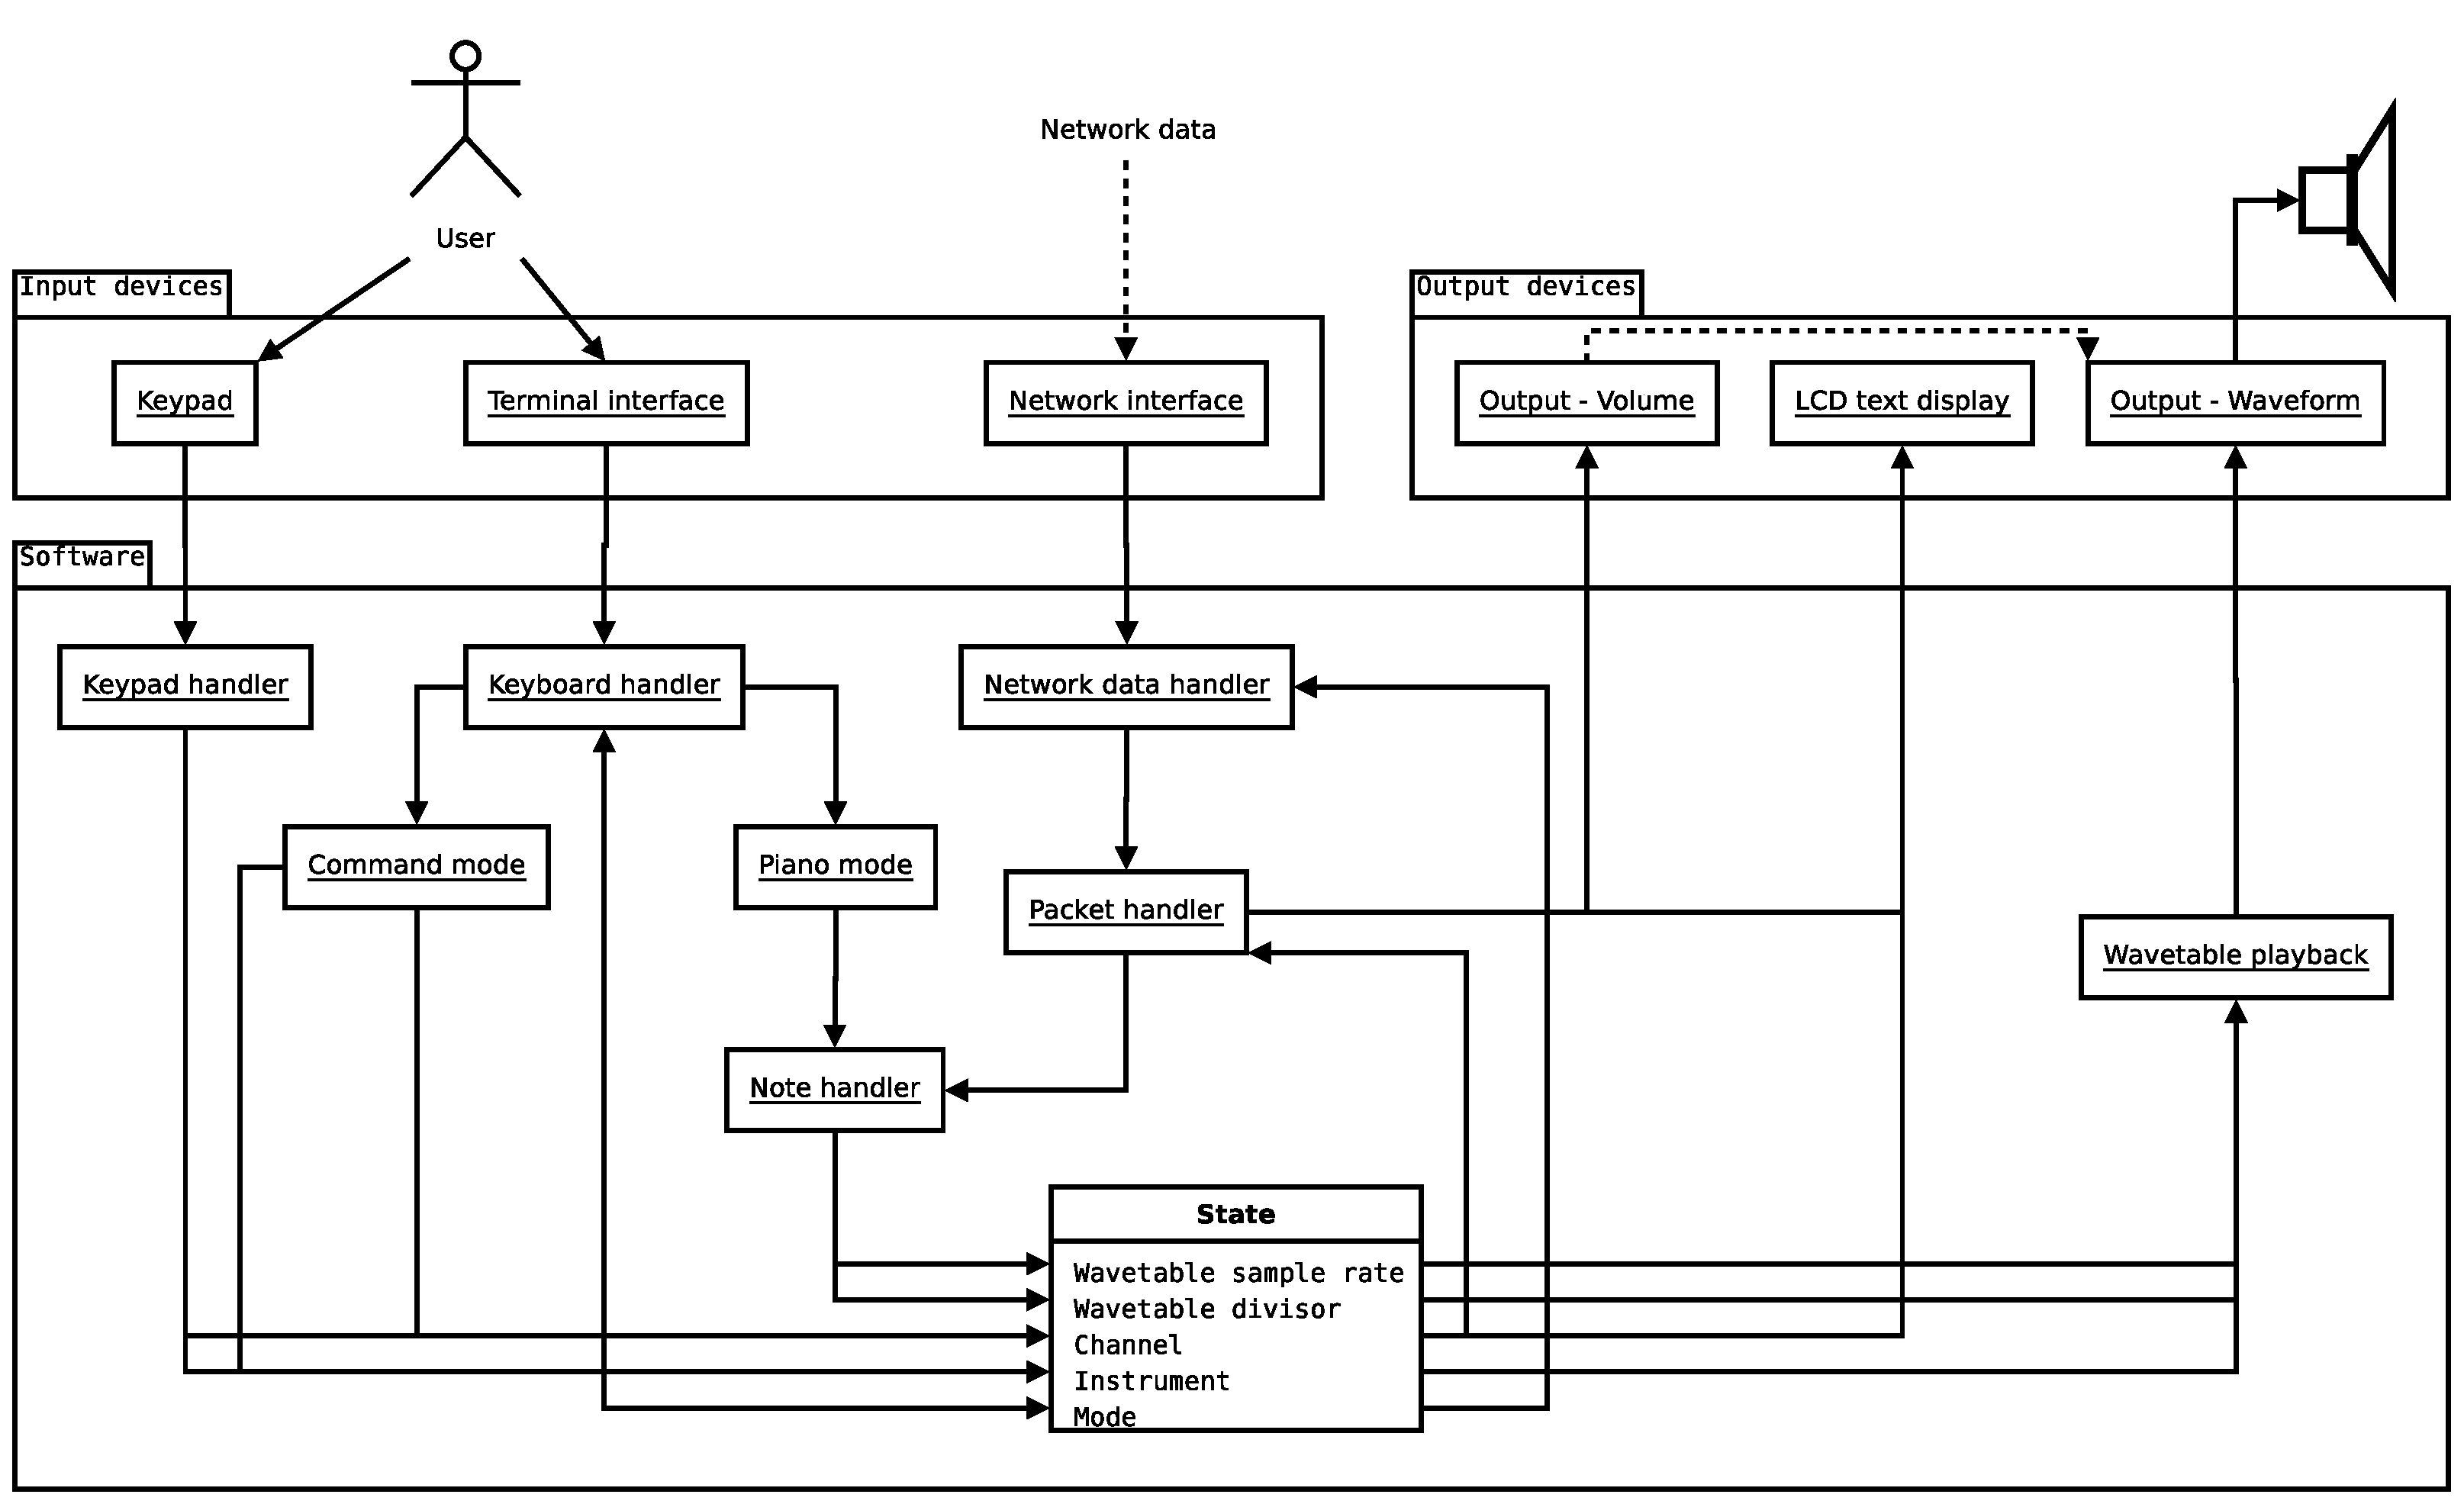
\includegraphics[totalheight=0.55\textheight,angle=90]{images/overview}
\caption{System Overview}\label{fig:systemoverview}
\end{figure}
\end{nowordcount}

The diagram in Figure \ref{fig:systemoverview} shows the conceptual architecture of my system.  The 
basic idea is that various inputs are processed and in some way modify the state of the system, and 
this state in turn affects the operation of the continuously-running wave table playback.

\section{Network Interface}
\label{sec:overview:network}

The network interface is a serial connection which receives a data stream at a rate of one 34-byte 
packet every $34ms$.  The data format is sixteen pairs of bytes, each pair containing a MIDI note 
value and a volume level (both in the range 0--127), with each pair representing a channel between 0 
and 15 (in order).  The packet is terminated with a null byte (00h) and a carriage return (0Dh).  
The mapping of channel identifiers to instruments is shown in Table \ref{tab:channelids}.  For the 
``Percussion'' channel, the volume level represents the particular percussion instrument to play 
rather than the volume at which to play it.

\begin{nowordcount}
\begin{table}[htbp]
\centering
\begin{tabular}{c | l}
ID & Instrument \\
\hline\hline
0 & Bass Guitar \\
1 & Cello \\
2 & Church Organ \\
3 & Piano \\
4 & Saxophone \\
5 & Melody \\
6 & Violin \\
7 & Trombone \\
8 & Trumpet \\
9 & French Horn \\
10 & Synth \\
11 & Electric Guitar \\
12 & Acoustic Guitar \\
13 & Flute \\
14 & Piccolo \\
15 & Percussion
\end{tabular}
\caption{Network data channels}\label{tab:channelids}
\end{table}
\end{nowordcount}

The network handler collects data from the incoming byte stream.  The bytes are counted, and the 
currently selected channel is used to decide which note/volume pair to store (see 
Section~\ref{sec:design:network-handler} for rationale on this design).  When the end of a packet is 
detected, the byte count is checked and the data discarded if the packet was incomplete.  The packet 
is also discarded if the system is not in ``network mode'' (see Section~\ref{sec:overview:state}).
If there is no reason to discard the packet, the data is used to set the playback state of the 
system.  The volume is converted to an 8-bit value (left-shifted) and output to the hardware, and 
also used to set the appropriate part of the LCD text display.  The note handler is run with the 
note value.

\section{Note Handler}
\label{sec:overview:note-handler}

The note handler ``receives'' a MIDI note value, and uses it to find the appropriate state 
information in a lookup tables.  Firstly, a playback lookup table is used to find the PRT value and 
divisor, which are written to the PRT reload register and divisor register used by the playback loop 
respectively.  Secondly, a display lookup table is used to find a 4-character representation of the 
note, which is written to the LCD text display.  See Section~\ref{sec:design:lookup-tables} for 
details of the lookup tables.

\section{Wavetable Playback}
\label{sec:overview:playback}

Wavetable playback is controlled by the PRT and divisor settings --- how these affect the note being 
played is explained in Section~\ref{sec:design:wavetables}.  Every time the playback routine is 
called, the next sample from the wavetable for the current instrument is sent to the output device.  
The PRT reload value controls how often the playback routine is called.  The ``divisor'' controls 
the step between samples --- for example, 1 means every sample, 3 means every third sample.  The 
wavetable playback is affected only by the state of the system, it is not directly called from 
anywhere.

\section{Keypad Handler}
\label{sec:overview:keypad}

Since the keypad has 16 possible values, when a button is pressed on the keypad, the value is used 
to set the channel and instrument selection to that value.  \todo{Expand this?}

\section{Terminal Interface}
\label{sec:overview:terminal}

The SBC is connected to a PC via a serial connection.  This allows the user to interact with the 
software over this connection using terminal software, such as Seyon.  The user interface provided 
over the serial terminal is purely additional functionality --- the essentials of playback and 
channel selection can be used without this interface.  The keyboard handler decides what should be 
done based on the mode and the key pressed.

\begin{figure}
\centering
\includegraphics[width=0.9\textwidth]{images/terminal-prompt}
\caption{Serial Terminal Prompt}\label{fig:terminal-prompt}
\end{figure}

\subsection{``Network Mode''}

In the default mode, there are three possible actions the user can perform 
(Figure~\ref{fig:terminal-prompt}):

\begin{description}
\item[Change instrument:] Change the current instrument without changing the channel being read.  
This is useful for demonstrating all of the instruments when not all channels have activity.
\item[Change channel:] Change the current channel without changing the instrument.  Useful for 
testing all of the channels when only one instrument sample has been loaded, also makes sense for 
this to be possible given the availability of the first action.
\item[Piano mode:] Enter piano mode, where keyboard input is mapped to changing the note.
\end{description}

\subsection{``Piano Mode''}

In piano mode, the currently selected octave combined with pressing a key determines the note to 
play (explained further in Section~\ref{sec:design:piano-mode}).  Figure~\ref{fig:piano-mode} shows 
how the keys are mapped --- the layout is based on the note layout on a piano.  Since there are four 
rows of normal characters on a standard keyboard I decided to map the current octave and the octave 
above.  The ``$+$'' and ``$-$'' keys can be used to change the current octave.  Pressing ``Ctrl+D'' 
exits piano mode, returning to network mode.

When a note key is pressed, the correct MIDI note is found (via lookup tables and the octave offset) 
and passed to the note handler (Section~\ref{sec:overview:note-handler}).

\begin{figure}
\centering
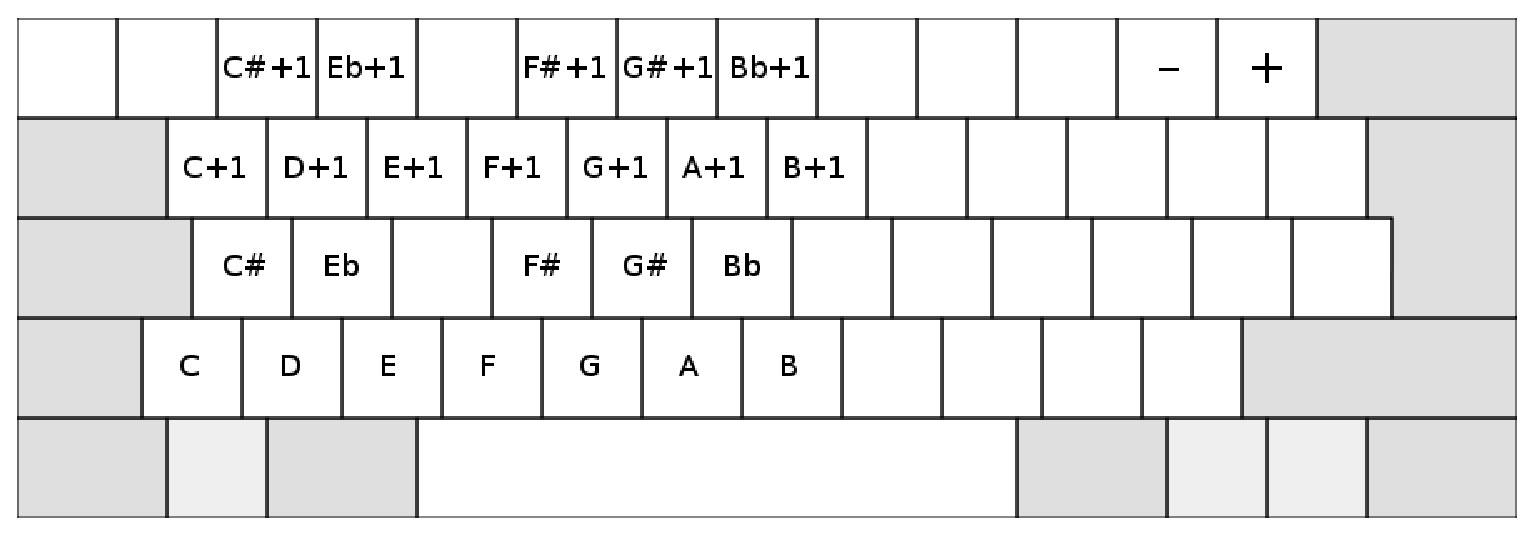
\includegraphics[width=0.9\textwidth]{images/piano-mode}
\caption{``Piano Mode'' Keyboard Layout}\label{fig:piano-mode}
\end{figure}

\section{State}
\label{sec:overview:state}

There are 5 main elements to the state of the system:

\begin{description}
\item[Wavetable sample rate:] The rate at which samples are read from the instrument wavetable and 
output.  This takes the form of the PRT reload value, and is one of two factors affecting the 
generated note frequency.
\item[Wavetable divisor:] The step size when reading from the instrument wavetable.  This is the 
second factor affecting the note frequency.  How these affect the frequency is explained in 
Section~\ref{sec:design:wavetables}.
\item[Channel:] The current channel being played.  This affects which data is used from the network 
stream, and the channel name being displayed on the LCD text display.
\item[Instrument:] The current instrument being used.  This affects which wavetable sample is being 
used by the playback routine.
\item[Mode:] The current system mode --- ``network'' or ``piano''.  This affects the actions of key 
presses on the terminal, and also whether or not network data is ignored.
\end{description}

% vim: fo=aw2tq tw=100 spell
\section{Design and Implementation}

\subsection{Audio output}
\label{sec:design:audio_output}

% TODO: sound/music theory somewhere?
The output device was jointly designed with my lab partner.  The most important property of any 
output device developed is obviously the ability to output a waveform that would audibly represent 
the intended musical note (and instrument).  However, since the network data also includes volume 
information, this needed to be taken into account.  This could be achieved in two ways:
\begin{enumerate}
\item Implementing a volume scaling function in software
\item Scaling the volume with more programmable hardware
\end{enumerate}
The first option has the advantage of giving the simplest, and therefore easiest, hardware to 
design.  Unfortunately, scaling the volume of a waveform during playback would involve modifying the 
amplitude of every step of a waveform with multiplication.  This would result in playback being a 
very processor-intensive task, which is fairly impractical for the speed and simplicity of our CPU.  
On the other hand, implementing volume scaling in hardware removes this burden from the CPU, freeing 
up the processing time for other tasks.

We chose to implement the volume scaling in hardware, and gave the hardware a very simple interface 
--- an 8-bit ``waveform'' input and an 8-bit ``volume'' input.  This would later make outputting a 
waveform a very fast software task --- one I/O operation per sample in the waveform, and one I/O 
operation for every volume value received.

The conversion from the two 8-bit values to the final audio signal can be described as a two-stage 
digital-to-analogue converter (DAC) with a final amplification stage.  A simple circuit of a DAC and 
inverting operational amplifier will give an output voltage between ground and $-V_{ref}$ 
proportional to the digital input, where $V_{ref}$ is the reference voltage of the DAC.  (The 
maximum output in practice is about $-V_{ref}\times0.85$.)  We decided to use this concept to 
develop a two-stage DAC consisting of two such circuits, where the output of the first became the 
$V_{ref}$ of the second.  The first becomes the ``volume'' DAC, effectively pre-scaling any signal 
output by the second, which would receive the waveform sample values.  Note that this design does 
not prevent the use of software scaling if desired, but gives the attractive possibility of avoiding 
it.

To interface with the SBC, the DAC inputs were connected to ports A and B of the parallel I/O 
controller.  Though the network data contained 7-bit volume values, and the hardware needed 8-bit 
values, we decided not to ``left-shift'' the data in hardware (wiring parallel I/O data pins 0--6 to 
DAC data pins 1--7) to maintain flexibility of the hardware.  (In my solution the volume values are 
left-shifted in software.)  The result of this was that existing I/O ports on the SBC were used, 
removing the need to create extra hardware for chip selection based on I/O address, and the DAC 
operation was simple because the parallel I/O is latched (data stays on the outputs between writes).

There are a few things worth noting in the circuit diagram for the audio output device (appendix 
\ref{appendix:circuit_diagram}):

\subsubsection{DACs In ``Flow-Through'' Mode}

The DAC0832 used for this project is a double-buffered digital to analogue converter.  Single 
buffering is generally useful for holding the input value in the DAC between writes.  Double 
buffering adds the ability to defer the write until some other signal --- this is especially useful 
in cases where several DACs need to change simultaneously but their data is received asynchronously, 
since the write between the first and second buffers can be triggered on all DACs at the same time.

In this instance however, the ``single-buffered'' effect is achieved through the parallel I/O having 
latched outputs, and the ``double-buffered'' effect is unneeded as the volume and waveform data are 
not directly related and do not need to be applied simultaneously.  By hard-wiring all of the 
signals related to writing and buffering to their ``enable'' value, the output of the DAC follows 
the digital input directly.  This means that writes to the parallel I/O have the effect of changing 
the DAC values instantly.

\subsubsection{DAC Potential Divider}

In the top-right of the circuit diagram there is a potential divider circuit between the $V_{ref}$ 
input of the volume DAC and $+12V$ (R1, R2 and C2).  It supplies a $\sim7.1V$ potential, made very 
smooth by the $22\mu{}F$ capacitor --- the DAC is very sensitive to noise on $V_{ref}$.

\subsubsection{Feedback Capacitors}

The capacitors C1 and C5 --- between the output and inverting input of both operational amplifiers) 
--- are to remove ``ringing'' and ``overshoot'' from the output signals (as recommended by the 
DAC0832 datasheet\cite{dac0832}).  Initially both capacitors were $68pF$, sufficient to remove any 
noticeable overshoot from the signal.  However, once the hardware and software solutions were 
complete and the maximum sample rate was known, the value of C5 was increased to $10nF$ to smooth 
the output signal and make it sound less ``square'' --- a problem present due to the quick value 
changes compared to the time between changes.

\subsubsection{Audio Amplifier}

The audio amplifier (IC5) is set up in a similar way to that described in the LM386 audio amplifier 
datasheet\cite{lm386} (diagram titled ``Amplifier with Gain = 20, Minimum Parts'') --- we were not 
too interested in voltage gain, our reason for using an amplifier was to supply more current so that 
driving a speaker did not result in clipping of the waveform.

\subsubsection{Pre-Amplifier Potential Divider}

The datasheet for the LM386\cite{lm386} states that the input voltage for the audio amplifier is 
$\pm0.4V$ --- above this voltage the signal is clipped (as we found through experimentation).  
However, the maximum output amplitude of the second DAC stage is $\sim5.1V$ ($7.1\times0.85^2$), so 
this needed to be brought within the acceptable input range of the LM386.  This was achieved with a 
potential divider comprising of a $150K\Omega$ resistor (R3) and a $10K\Omega$ potentiometer (P1).  

The potentiometer was used to give a ``physical'' volume control to the system.  The $220\mu{}F$ 
capacitor (C6) before the potential divider AC-couples the signal, putting it in the range 
$\sim\pm2.55V$.  When the potentiometer is at it's maximum resistance, the signal into the LM386 is 
in the range $\sim\pm0.16V$.  This is actually lower than necessary, because when I calculated the 
resistor values I failed to take into account the AC coupling (I was aiming for a maximum voltage of 
$\pm0.32V$).  However, this is of little consequence since the maximum output can still cause the 
amplifier to clip.


\subsection{Keypad handler}
\label{sec:design:keypad_handler}

The keypad is an awkward device for trying to get a single value from --- it interrupts continuously 
for the duration of the key press.  When implementing the keypad handler, this was the main problem 
I had to overcome.

My solution was to create a kind of lockout for that particular interrupt handler.  The result is a 
variable that acts as an ``already handled'' flag for keypad interrupts.  When a keypad interrupt 
happens, the flag is checked --- if it's non-zero, then the interrupt gets effectively ignored.  If 
it's zero, the interrupt handler executes as normal.  At the end of the interrupt handler, there are 
a few NOP (no operation) instructions before setting the lockout variable back to zero and returning 
from the interrupt, but \emph{after} the interrupts are re-enabled.  The idea is that if the key is 
still pressed, it will interrupt during those NOPs, before the flag is cleared, and those interrupts 
will get ignored, but on the very last interrupt it will complete the handler.  This completely 
eliminates the possibility of accidental repeats.

For comparison, the alternative solution was to insert a delay after handling the keypress to allow 
time for the key to be released.  I found this method to be less than ideal, since if the delay is 
too long it can result in the system seeming unresponsive, and if too short then repeated interrupts 
can occur.  I felt it was better to maintain a direct response between action and reaction.

\subsection{Note lookup tables}
\label{notelookuptables}

Lookup tables are needed to contain the PRT value, divisor and note name (including octave) for 
every MIDI note.  The note names are in a separate lookup table to the other data as having an LCD 
information display was a lower priority than working sound playback and was implemented much later.

% TODO: expand on comparison of formats
The most efficient way to use a lookup value for a table is to multiply it by a power of two (left 
shifting), so blocks of data in the lookup table are also going to be $2^n$ bytes long.  However, 
the data for note playback is 3 bytes (a 16-bit PRT value plus an 8-bit divisor), so I was faced 
with the choice of having two lookup tables for the playback data or wasting $\frac{1}{4}$ of the 
space used by the table.  After writing the necessary assembler for reading from both possible 
formats and analysing their execution times, I found that the single table method resulted in faster 
code.  Combined with the fact I was not under pressure to conserve memory, I chose the single table 
method.

% TODO: expand on the result sorting
The Python script\footnote{"tools/pitchtable.py" in the submitted source code} I wrote to generate 
the lookup tables\footnote{"note\_lookup.s"} is based on the concept outlined in \ref{wavetables} 
for creating new frequencies from a single sample by modifying the sample rate and divisor.  PRT and 
divisor values are calculated for the frequency information in the pitch 
table\footnote{"tools/pitchtable.csv" - octave, MIDI note number, note name, frequency}.

The first step is calculating the PRT value for every divisor, $D$ from 1 to 255, first by 
calculating the sample rate using

\[R_{target} = \frac{F_{target} \times R_{source}}{F_{source} \times D}\]

(rearranged from a similar equation in \ref{wavetables}) and then converting this to a PRT value 
using

\[PRT = round\left(\frac{F_{CPU}}{D_{PRT}\times{}R_{target}}\right)\]

where $F_{CPU}$ is the CPU frequency (6,144,000) and $D_{PRT}$ is the PRT divisor (20).  Because the 
result has been rounded to the nearest integer, the effective frequency will be different to the 
desired frequency.  The effective frequency is calculated by using the $PRT$ and $R_{target}$ 
calculations in reverse:

\[F_{effective} = \frac{F_{source}\times{}D\times{}\frac{F_{CPU}}{D_{PRT}\times{}PRT}}{R_{source}}\]

The error, E is calculated with the following, giving a value in the range 0--1:

\[E = \frac{\left|F_{effective} - F_{target}\right|}{F_{target}}\]

% TODO: to joke or not to joke?
For each note, the results for all the divisors are collected together, discarding those where the 
sample rate is higher than 8kHz (a sensible limit given the CPU speed), and sorted in reverse order 
by $R^{1-E}$.  The idea is that the basic ordering aims for a high sample rate, but any kind of 
significant error greatly diminishes the value of the result.  The first result is taken from the 
sorted list, giving the PRT and divisor values the algorithm decides best represent the frequency.  
While almost seeming like mathematical voodoo, the worst error rate for any note in the resulting 
table is $1.13\%$, with an average sample rate of just under 7kHz.  Other sorting methods I tried 
had varied results, generally creating high sample rates with high error margins, or low error 
margins with bad sample rates.

The format of the resulting lookup table is:
\begin{nowordcount}
\begin{center}
\begin{tabular}{c | c | c | c | c}
Byte & 0 & 1 & 2 & 3 \\
\hline
Usage & PRT low & PRT high & Divisor & 00h \\
\end{tabular}
\end{center}
\end{nowordcount}

The script also produces a second table which contains a 4-character representation of the note 
created from the octave number and note name.

% vim: fo=aw2tq tw=100 spell
\section{Testing and Evaluation}

% vim: fo=aw2tq tw=100 spell
\chapter{Technical Specification}

\section{Operating Parameters}

\begin{itemize}
\item Power supply: $+12V$, $-12V$, $+5V$, Ground
\item Temperature: 0--70$^{\circ}$C\footnote{Minimum range suitable for all components.}
\end{itemize}

\section{Functionality}
\label{sec:spec:functionality}

\subsection{Audio Playback}

\begin{itemize}
\item Playable MIDI notes
    \begin{itemize}
    \item Maximum range: 0--127
    \item Optimal range: 0--106
    \item Accuracy (worst): $\pm1.13\%$
    \item Accuracy (avg.): $\pm0.5\%$
    \end{itemize}
\item Volume range
    \begin{itemize}
    \item 128 steps
    \item Linear scale
    \item Additional hardware volume control
    \end{itemize}
\item Supported instruments
    \begin{itemize}
    \item Bass guitar
    \item Cello
    \item Church Organ
    \item Piano
    \item Saxophone
    \item Melody
    \item Violin
    \item Trombone
    \item Trumpet
    \item French Horn
    \item Synth
    \item Electric Guitar
    \item Acoustic Guitar
    \item Flute
    \item Piccolo
    \end{itemize}
\end{itemize}

\subsection{Interface}
\begin{itemize}
\item Network stream
    \begin{itemize}
    \item 19,200bps baud rate
    \item 34-byte packet length
        \begin{itemize}
        \item 2 bytes per channel, in order --- pitch, volume
        \item Terminated by null and carriage return (00h, 0Dh)
        \end{itemize}
    \end{itemize}
\item 16-button keypad --- allows changing of channel at any time.
\item Terminal interface
    \begin{itemize}
    \item Change channel and instrument independently.
    \item Piano mode for manually playing notes with a keyboard --- layout based on an actual piano.
    \item Not necessary for operation --- system can be used standalone.
    \end{itemize}
\end{itemize}


\section{Cost}
\label{sec:spec:cost}

\begin{nowordcount}
\begin{center}
\begin{tabular}{c | c | r | r}
Part & Quantity & Per-unit & Total \\
\hline\hline
64180 SBC               & 1     & \pounds100.00 & \pounds100.00 \\
DAC0832LCN              & 2     & \pounds1.66 & \pounds3.32 \\
LM356N                  & 2     & \pounds0.40 & \pounds0.80 \\
LF386N-1                & 1     & \pounds0.26 & \pounds0.26 \\
$8\Omega$ speaker       & 1     & \pounds2.62 & \pounds2.62 \\
$10K\Omega$ potentiometer & 1     & \pounds0.72 & \pounds0.72 \\
Metal film resistor ($\pm1\%$)    & 3     & \pounds0.06 & \pounds0.18 \\
Electrolytic capacitor  & 5     & \pounds0.08 & \pounds0.40 \\
Ceramic capacitor       & 5     & \pounds0.07 & \pounds0.35 \\
PCB manufacture (40mm $\times$ 40mm) & 1     & \pounds2.90 & \pounds2.90 \\
\hline
\multicolumn{3}{r |}{\textbf{Total}} & \textbf{\pounds111.15} \\
\end{tabular}
\end{center}
\end{nowordcount}

Component prices (except for SBC) quoted from Farnell UK.  PCB manufacture quoted from PCBTrain 
quote calculator\footnote{\url{http://www.pcbtrain.co.uk/onestepquote.php}}.  Prices correct as of 
07/04/2008.  Based on a batch of 100 units.

% vim: fo=aw2tq tw=100 spell
\chapter{Further Work}

\section{Note lookup tables}
Since the major use of the note lookup tables is by the network handler, which uses all values of 
both tables, given a little more time it would make sense to combine the playback and display 
information into a single lookup table.  The new lookup table would contain blocks of 8 bytes, 
however the data only amounts to 7 bytes.  This would actually be useful, as the 8th byte would be 
set to 00h, which is the string terminator used by "lcd_print"\footnote{Line 48 of "lcd.s"}.  If the 
new lookup table format was

\begin{nowordcount}
\begin{center}
\begin{tabular}{r || c | c | c | c | c | c | c | c}
Byte & 0 & 1 & 2 & 3 & 4 & 5 & 6 & 7 \\
\hline
Usage & PRT low & PRT high & Divisor & \multicolumn{4}{c |}{LCD info.} & 00h \\
\end{tabular}
\end{center}
\end{nowordcount}

the relevant section\footnote{Lines 471--519 of "synth.s"} of the network packet handler might look 
more like this:

\begin{nowordcount}
\begin{h180}
# (MIDI note is already in L)
# Multiply by 8 to address 8-byte blocks
ld h, 0x08
mlt hl
# Perform lookup (offset from base address)
ld de, notedata_lookup
add hl, de
# Low PRT byte
ld a, (hl)
out0 (PRT0_RLD_L), a
# High PRT byte
inc hl
ld a, (hl)
out0 (PRT0_RLD_H), a
# Divisor
inc hl
ld a, (hl)
# Store the divisor in the shadow register (interrupts
# disabled to prevent double-swapping)
di
exx
ld c, a
exx
ei
# Set the location on the LCD
ld a, LCD_NOTE
call lcd_setlocation
# Output the note name
inc hl
call lcd_print
\end{h180}
\end{nowordcount}


\section{Alternative Design}

During the late stages of the project I started development of an alternative design, which I 
abandoned due to time constraints.  The idea was that instead of the current software processing and 
output of samples from a wavetable, I would create hardware that could be programmed with an 
instrument number and note and would play the correct sound at the correct frequency.   This would 
leave the CPU with only network data and visual output to handle, but would also allow the extra CPU 
time to be used for other functions, such as an advanced visualisation on an liquid crystal matrix 
display.

My rudimentary ideas for this included the following:

\begin{itemize}
\item A ROM chip containing all of the wavetable samples (probably at 256 bytes per instrument).
\item An 8-bit counter connected to the lowest 8 bits of the wavetable ROM address for stepping 
through the instrument sample.
\item A 4-bit register connected to the next 4 bits of the wavetable address for selecting the 
instrument.
\item A 16-bit programmable reload timer running at a clock divider of 2, for controlling the 
playback frequency --- the output of this is the clock for the 8-bit address counter.  (Plus two 
8-bit registers to store the reload value.)
\item A note lookup table in software for the PRT values.
\end{itemize}

I built and experimented with the PRT section of this idea, and could successfully generate 
frequencies between 46.875Hz and 3.072MHz when using a system clock of 6.144MHz, by setting the 
reload value manually using two 8-bit DIP switches.
% TODO: continue this section


\appendix

\begin{nowordcount}

\chapter{Circuit diagram}
\begin{center}
\label{appendix:circuit_diagram}
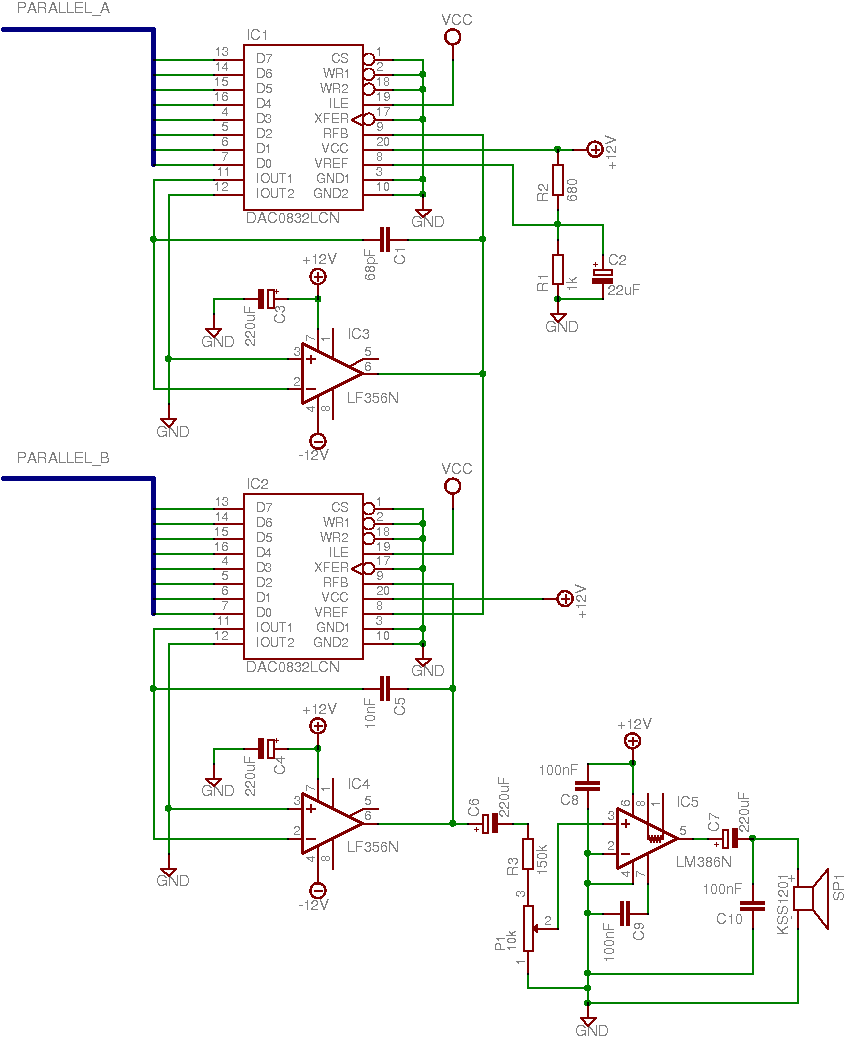
\includegraphics[width=0.95\textwidth]{images/output-schematic}
\end{center}

\chapter{Lookup Table Performance Comparison}
\label{appendix:lookup-table-comparison}
\lstinputlisting[language=h180]{../notes/changenote-analysis.s}

\pagebreak
\begin{thebibliography}{99}
% \bibitem{ref}Author:
% \emph{Title},
% \url{http://} (year)

\bibitem{lm386}National Semiconductor:
\emph{LM386 Low Voltage Audio Power Amplifier}
\url{http://www.national.com/ds.cgi/LM/LM386.pdf} (2000)

\bibitem{dac0832}National Semiconductor:
\emph{DAC0830/DAC0832 8-bit $\mu$P Compatible, Double-Buffered D to A Converters}, 
\url{http://www.national.com/ads-cgi/viewer.pl/ds/DA/DAC0830.pdf} (2002)

\bibitem{lf356}National Semiconductor:
\emph{LF155/LF156/LF256/LF257/LF355/LF356/LF357 JFET Input Operational Amplifiers},
\url{http://www.national.com/ds.cgi/LF/LF155.pdf} (2001)
\end{thebibliography}

\end{nowordcount}

\end{document}
